% !TEX program = pdflatex
% Presentation superviseur -- Week 2 -- 2026-04-21
% Knowledge Graph juridique francais -- Benchmarks + Graphes

\documentclass[aspectratio=169,10pt]{beamer}

\usepackage[utf8]{inputenc}
\usepackage[T1]{fontenc}
\usepackage[french]{babel}
\usepackage{lmodern}
\usepackage{booktabs}
\usepackage{array}
\usepackage{tikz}
\usepackage{xcolor}
\usepackage{graphicx}
\usetikzlibrary{positioning, arrows.meta, shapes.geometric, fit, backgrounds}

\usetheme{Madrid}
\usecolortheme{seahorse}
\setbeamertemplate{navigation symbols}{}
\setbeamertemplate{footline}[frame number]
\setbeamerfont{footnote}{size=\tiny}

% Couleurs custom (identiques Week 1)
\definecolor{accent}{RGB}{41, 92, 155}
\definecolor{accentsoft}{RGB}{230, 238, 247}
\definecolor{warn}{RGB}{200, 80, 40}
\definecolor{ok}{RGB}{30, 130, 70}

% Boxes
\newcommand{\keybox}[1]{%
  \begin{center}
  \colorbox{accentsoft}{\parbox{0.92\linewidth}{\centering #1}}
  \end{center}}

% Metadata
\title[KG juridique FR --- Week 2]{Construction d'un Knowledge Graph juridique français}
\subtitle{Point d'avancement --- Week 2 : benchmarks \& graphes}
\author{Matthieu Kaeppelin}
\institute{Stage FE Recherche}
\date{21 avril 2026}

\begin{document}

% ============================================================
\begin{frame}
  \titlepage
\end{frame}

% ============================================================
\begin{frame}{Plan}
  \tableofcontents
\end{frame}

% ============================================================
\section{Rappel du besoin et de la question}

\begin{frame}{Rappel du besoin}
  \keybox{\small Un juriste qui répond à une question de droit doit mobiliser : des \textbf{articles} (règles), des \textbf{arrêts} (jurisprudence) et une \textbf{démonstration} qui relie les deux aux faits du dossier.}

  \vspace{0.5em}
  \textbf{Outil cible}
  \begin{itemize}\footnotesize
    \item Pour une question juridique donnée, retrouver automatiquement :
    \begin{itemize}\footnotesize
      \item les \textbf{articles pertinents}
      \item la \textbf{jurisprudence applicable} (y compris les arrêts contraires)
      \item une \textbf{réponse traçable et justifiée}
    \end{itemize}
    \item Pour : avocats, magistrats, juristes d'entreprise, particuliers
  \end{itemize}

  \vspace{0.5em}
  \textbf{Question de recherche}
  \keybox{\small Dans quelle mesure une architecture \textbf{GraphRAG} peut-elle améliorer la recherche juridique française en termes de \textbf{pertinence}, \textbf{performance} et \textbf{explicabilité} ?}
\end{frame}

\begin{frame}{Pourquoi le RAG vectoriel ne suffit pas}
  \begin{columns}[T]
    \column{0.5\textwidth}
    \textbf{Limites du RAG vectoriel sur le droit}
    \begin{itemize}\footnotesize
      \item La recherche juridique est \textbf{multi-saut} : article $\to$ arrêt $\to$ article cité $\to$ JP interprétative
      \item Un arrêt qui \textbf{revire} une jurisprudence est sémantiquement opposé à l'ancien : le vectoriel les rapproche mal
      \item Le RAG ramène des chunks "proches du sens", pas des \textbf{liens institutionnels}
    \end{itemize}

    \column{0.5\textwidth}
    \textbf{Ce qu'apporte un graphe}
    \begin{itemize}\footnotesize
      \item Liens \textbf{explicites} entre arrêts (cite, confirme, casse, rapproche)
      \item Liens \textbf{explicites} entre arrêts et articles
      \item Permet la \textbf{navigation} et le \textbf{raisonnement multi-saut}
      \item Support naturel pour la \textbf{traçabilité}
    \end{itemize}
  \end{columns}

  \vspace{0.5em}
  \keybox{\small Pour prouver cet apport, on doit d'abord \textbf{mesurer} la performance des systèmes existants sur la tâche. D'où la priorité : construire un benchmark.}
\end{frame}

% ============================================================
\section{Architecture cible du benchmark}

\begin{frame}{Architecture du benchmark --- 6 modules $\times$ 5 configurations}
  \textbf{6 modules couvrant les 2 niveaux de raisonnement juridique}

  \vspace{0.2em}
  \footnotesize
  \renewcommand{\arraystretch}{1.1}
  \begin{tabular}{@{}p{2cm} p{5.5cm} p{6.5cm}@{}}
    \toprule
    \textbf{Niveau} & \textbf{Modules} & \textbf{Tâche type} \\
    \midrule
    Principe    & M1 (Principe QA), M3 (Multi-saut), M4 (QCM), M5 (Temporalité) & "Quelles sont les conditions de X ?" \\
    Application & M2 (Applied QA), M6 (Interprétation arrêt $\star$) & "Dans mon dossier, X est-il valable ?" \\
    \bottomrule
  \end{tabular}

  \vspace{0.8em}
  \textbf{5 configurations à benchmarker sur chaque module}

  \vspace{0.3em}
  \footnotesize
  \begin{tabular}{@{}l l l@{}}
    \toprule
    \textbf{\#} & \textbf{Configuration} & \textbf{Ce qu'on mesure} \\
    \midrule
    B1 & LLM seul (zero-shot)                 & Connaissance intrinsèque \\
    B2 & LLM + RAG vectoriel                  & Apport retrieval vectoriel \\
    B3 & LLM multi-step agentique (sans RAG)  & Apport chaîne de pensée \\
    B4 & LLM + RAG + agentique                & État de l'art "classique" \\
    \textbf{C}  & \textbf{LLM + GraphRAG (notre cible)} & \textbf{Apport du graphe structuré} \\
    \bottomrule
  \end{tabular}
\end{frame}

\begin{frame}{Sources du benchmark par module}
  \footnotesize
  \renewcommand{\arraystretch}{1.2}
  \begin{tabular}{@{}l p{5.5cm} p{6cm}@{}}
    \toprule
    \textbf{Module} & \textbf{Source principale} & \textbf{Statut} \\
    \midrule
    M1 --- Principe QA          & Les-Audits-Affaires (LegMLAI, 2\,670 cas FR, 9 codes) & Dataset public réutilisable \\
    M1' --- CRFPA (complément)  & Sujets + grilles CNB + copies IEJ Strasbourg & \textbf{À construire cette semaine} \\
    M2 --- Applied QA           & Cases synthétiques (Hector) + construction manuelle & En cours \\
    M3 --- Multi-saut           & Champ \texttt{rapprochements} Judilibre & \textbf{À construire cette semaine} \\
    M4 --- QCM                  & Génération auto depuis le graphe & Prévu \\
    M5 --- Temporalité          & Articles abrogés + revirements & Prévu (nécessite KG versionné) \\
    M6 --- Interprétation arrêt & Cases Hector + annotation à 7 dimensions & 5 cas gold MVP déjà livrés \\
    \bottomrule
  \end{tabular}

  \vspace{0.5em}
  \keybox{\small Objectif semaine 2 : produire les livrables pour \textbf{M1' et M3} + poser l'\textbf{infrastructure graphe} nécessaire à M3, M4, M5 et à la configuration C.}
\end{frame}

% ============================================================
\section{Sources mobilisées et exploration}

\begin{frame}{Sources mobilisées pour construire M1' --- CRFPA}
  \begin{center}
  \textbf{Point de départ}
  \end{center}

  \keybox{\small Depuis 2025, le \textbf{Conseil National des Barreaux} publie les \textbf{grilles de notation officielles} de ses épreuves écrites.}

  \vspace{0.3em}
  \begin{columns}[T]
    \column{0.55\textwidth}
    \textbf{Trois sources officielles complémentaires}
    \begin{itemize}\footnotesize
      \item \textbf{Sujets CNB} 2024 + 2025 \\ (12 épreuves $\times$ 2 ans = 24 énoncés)
      \item \textbf{Grilles officielles CNB} \\ (points attendus par le jury)
      \item \textbf{Meilleures copies IEJ Strasbourg} (2022-2025)
    \end{itemize}

    \column{0.45\textwidth}
    \textbf{Triplet exploitable}
    \vspace{0.3em}
    \begin{center}
    \scriptsize
    Sujet CNB $\rightarrow$ définit la question \\
    Grille CNB $\rightarrow$ définit la rubrique attendue \\
    Copies IEJ $\rightarrow$ confirment articles + JP utilisés
    \end{center}

    \vspace{0.3em}
    \small\textit{$\Rightarrow$ Ground truth validée par le jury national, sans annotation manuelle.}
  \end{columns}
\end{frame}

\begin{frame}{Sources mobilisées pour construire M3 --- rapprochements Judilibre}
  \textbf{Ce que la base Judilibre contient (déjà enrichie)}
  \begin{itemize}\footnotesize
    \item \textbf{553\,075 arrêts de la Cour de cassation} (complétée par CA et TJ pour un total de 1{,}1\,M)
    \item Champ \texttt{rapprochements} : d'autres arrêts que la Cour \textbf{déclare à mettre en regard}
    \item Champ \texttt{code\_article\_pairs} : articles cités, au format canonique \texttt{code\_civil:1240}
  \end{itemize}

  \vspace{0.3em}
  \keybox{\small Le champ \texttt{rapprochements} Judilibre = \textbf{ground truth institutionnelle gratuite} pour la tâche \textit{"navigation entre JP liées"}.}

  \vspace{0.3em}
  \textbf{Format du \texttt{rapprochement.title} (seul champ rempli)}
  \begin{block}{\scriptsize Exemple}
    \scriptsize\texttt{"Crim., 18 janvier 2011, pourvoi n° 10-87.525, Bull. crim. 2011, n° 7 (cassation)."}
  \end{block}
  \footnotesize\textit{Extraction par regex sur le numéro de pourvoi $\rightarrow$ matching ensembliste.}

  \vspace{0.3em}
  \textbf{Sources doctrinales} (Actu-Juridique, Village-Justice) : évaluées, reportées à Phase 2 --- gain marginal vs coût d'annotation pour un MVP.
\end{frame}

% ============================================================
\section{Méthodologie adoptée}

\begin{frame}{Méthodologie --- format de ground truth}
  \textbf{Rubrique hiérarchisée à 3 strates}

  \vspace{0.2em}
  Inspirée de HealthBench (OpenAI 2025) et PLawBench (Shi \textit{et al.} 2026).

  \footnotesize
  \begin{tabular}{@{}l l p{9cm}@{}}
    \toprule
    \textbf{Strate} & \textbf{Poids} & \textbf{Signification} \\
    \midrule
    \texttt{core}     & 3 & Un étudiant L2 doit les citer --- "le système répond juste" \\
    \texttt{expected} & 2 & Attendu d'un praticien --- "le système répond bien" \\
    \texttt{expert}   & 1 & Navigation KG profonde --- "le système exploite la structure" \\
    \bottomrule
  \end{tabular}

  \vspace{0.4em}
  \textit{Score composite} $=\frac{3 \cdot \mathrm{cov}_{\mathrm{core}} + 2 \cdot \mathrm{cov}_{\mathrm{expected}} + \mathrm{cov}_{\mathrm{expert}}}{\mathrm{total\_weight}}$

  \vspace{0.4em}
  \keybox{\small Discrimine structurellement : un RAG vectoriel plafonne sur \texttt{core + expected}, un GraphRAG doit décrocher sur \texttt{expert}.}
\end{frame}

\begin{frame}{Méthodologie --- triangulation anti-biais}
  \textbf{Problème à éviter : le biais circulaire}

  \vspace{0.2em}
  Si un LLM génère la ground truth \textit{et} qu'un LLM y est évalué, on mesure la cohérence du modèle avec lui-même, pas sa justesse.

  \vspace{0.4em}
  \textbf{Solution : triangulation par sources externes}

  \vspace{0.2em}
  \begin{center}
  \begin{tikzpicture}[scale=0.9, transform shape,
      src/.style={rectangle, rounded corners, draw=accent, fill=accentsoft, thick, minimum width=2.8cm, minimum height=0.7cm, font=\small},
      llm/.style={rectangle, draw=accent!80, thick, minimum width=2.5cm, minimum height=0.7cm, font=\small},
      out/.style={rectangle, rounded corners, draw=ok, fill=green!8, thick, minimum width=3cm, minimum height=0.7cm, font=\small}]

    \node[src] (s1) at (0,2)   {Sujet CNB};
    \node[src] (s2) at (0,1)   {Grille officielle CNB};
    \node[src] (s3) at (0,0)   {Copies IEJ};

    \node[llm] (llm) at (5,1)  {LLM (Opus)};
    \node[out] (r)   at (9.5,1) {Rubrique structurée};

    \draw[-{Stealth}, thick] (s1.east) -- (llm.west);
    \draw[-{Stealth}, thick] (s2.east) -- (llm.west);
    \draw[-{Stealth}, thick] (s3.east) -- (llm.west);
    \draw[-{Stealth}, thick] (llm) -- (r);
  \end{tikzpicture}
  \end{center}

  \vspace{0.2em}
  \textbf{Résultat} : pour le benchmark CRFPA, \textbf{92\,\% des points de rubrique} sont \textit{sourcés externe} (grille jury ou copie étudiante), \textbf{8\,\% seulement} sont LLM-intrinsèques.
\end{frame}

% ============================================================
\section{Tests de validation}

\begin{frame}{Tests de validation (1/2)}
  \textbf{Test 1 --- Orchestration multi-LLM pour CRFPA}
  \begin{itemize}\footnotesize
    \item 10 subagents Opus en parallèle (1 par matière)
    \item Taux de réussite au premier coup : 50\,\%
    \item Rattrapage par relance ciblée $\to$ 100\,\% de complétion
    \item Temps total : $\sim$6\,h d'orchestration pour 11 matières
  \end{itemize}

  \vspace{0.5em}
  \textbf{Test 2 --- Détection d'un biais circulaire}
  \begin{itemize}\footnotesize
    \item Première version "droit des obligations" générée \textit{sans} triangulation : \textcolor{warn}{\textbf{100\,\% des rubriques LLM-intrinsèques}}
    \item Biais détecté \textbf{avant dissémination}
    \item Refonte avec triangulation $\to$ \textcolor{ok}{\textbf{8\,\% seulement}}
  \end{itemize}

  \keybox{\small Ce test a \textbf{débloqué} le reste de la semaine : sans ce filtre, le benchmark aurait été inutilisable.}
\end{frame}

\begin{frame}{Tests de validation (2/2)}
  \textbf{Test 3 --- Parse rate des rapprochements Judilibre}
  \begin{itemize}\footnotesize
    \item Sur échantillon récent (2020-2024) : 80\,\% de rapprochements parsables par regex
    \item Sur corpus complet : 16{,}3\,\% (les titres pré-1980 ne suivent pas le format \texttt{pourvoi n° XX-XX.XXX})
    \item \textbf{Limite de la donnée brute}, pas de la regex --- documenté comme biais connu
  \end{itemize}

  \vspace{0.5em}
  \textbf{Test 4 --- Performance de la visualisation}
  \begin{itemize}\footnotesize
    \item Spring-layout NetworkX sur 31\,k n\oe uds $\to$ $\sim$10\,min CPU
    \item Acceptable en préparatoire, prohibitif en temps réel
    \item À anticiper pour les expériences à grande échelle
  \end{itemize}
\end{frame}

% ============================================================
\section{Livrable 1 --- Benchmark CRFPA (M1')}

\begin{frame}{Livrable 1 --- Benchmark CRFPA}
  \keybox{\small Couvre le niveau \textbf{Principe QA} sur un corpus \textbf{examinal CNB officiel}.}

  \begin{columns}[T]
    \column{0.45\textwidth}
    \textbf{Chiffres}
    \vspace{0.2em}
    \footnotesize
    \begin{tabular}{@{}l r@{}}
      \toprule
      Questions & \textbf{38} \\
      Matières & 11 \\
      Points de rubrique & 681 \\
      \quad \texttt{core}     & 294 \\
      \quad \texttt{expected} & 181 \\
      \quad \texttt{expert}   & 206 \\
      Articles uniques & 296 \\
      JP uniques & 188 \\
      \bottomrule
    \end{tabular}

    \column{0.55\textwidth}
    \textbf{Distribution des sources}
    \vspace{0.2em}
    \footnotesize
    \begin{tabular}{@{}l r@{}}
      \toprule
      Grille CNB (jury officiel) & 52\,\% \\
      Copies IEJ Strasbourg & 40\,\% \\
      LLM-intrinsèque (résiduel) & 8\,\% \\
      \bottomrule
    \end{tabular}

    \vspace{0.5em}
    \textbf{Matières couvertes}
    \begin{itemize}\scriptsize
      \item Obligations, Civil, Pénal, Affaires, Social, Administratif, Fiscal, International/Européen
      \item Procédures civile, pénale, administrative
    \end{itemize}
  \end{columns}

  \vspace{0.5em}
  \textbf{Limites identifiées}
  \begin{itemize}\footnotesize
    \item 100\,\% des JP portent \texttt{uncertainty\_note} $\to$ validation Judilibre requise avant usage
    \item Copies IEJ = scans manuscrits $\to$ \texttt{tesseract-fra} requis pour scale-up
  \end{itemize}
\end{frame}

% ============================================================
\section{Livrable 2 --- Benchmark Rapprochements (M3)}

\begin{frame}{Livrable 2 --- Benchmark Rapprochements}
  \keybox{\small Étant donné un arrêt Cass (référence + texte intégral) $\to$ lister les \textbf{rapprochements officiels} que la Cour elle-même a déclarés.}

  \begin{columns}[T]
    \column{0.5\textwidth}
    \textbf{Pipeline} (3 passes streaming)
    \begin{itemize}\footnotesize
      \item Pass 1 : scan + filtrage (${\geq}3$ rapprochements parsables)
      \item Pass 2 : index inverse \texttt{pourvoi\_norm $\to$ id\_Judilibre}
      \item Pass 3 : résolution + stratification + export
    \end{itemize}

    \vspace{0.2em}
    \textbf{Durée totale : $<$ 1 minute} (sur 5\,Go).

    \column{0.5\textwidth}
    \textbf{Chiffres}
    \vspace{0.2em}
    \footnotesize
    \begin{tabular}{@{}l r@{}}
      \toprule
      Arrêts CC scannés & 553\,075 \\
      Questions produites & \textbf{1\,532} \\
      Rapprochements en GT & 5\,832 \\
      Taux de résolution vers ID & 98{,}7\,\% \\
      \bottomrule
    \end{tabular}
  \end{columns}

  \vspace{0.5em}
  \textbf{Stratification par chambre}

  \scriptsize
  Soc. 375 $\cdot$ Crim. 370 $\cdot$ Civ. 2e 291 $\cdot$ Civ. 1re 236 $\cdot$ Civ. 3e 181 $\cdot$ Com. 39 $\cdot$ Ass. plén. 26 $\cdot$ Ch. mixte 10
\end{frame}

\begin{frame}{Les deux benchmarks se complètent}
  \footnotesize
  \begin{tabular}{@{}p{3.2cm} p{5.2cm} p{5.5cm}@{}}
    \toprule
    \textbf{Axe} & \textbf{Benchmark CRFPA (M1')} & \textbf{Benchmark Rapprochements (M3)} \\
    \midrule
    Tâche         & QA juridique structurée           & Recommandation de JP liées \\
    Ground truth  & Rubrique CNB + copies IEJ         & Rapprochements Cass officiels \\
    Mesure        & Qualité du raisonnement           & Navigation entre décisions \\
    \textbf{Discriminant cible} & \textbf{RAG vs LLM seul} & \textbf{Graphe vs RAG vectoriel} \\
    Taille        & 38 Q (qualité max)                & 1\,532 Q (volume + officiel) \\
    Ancrage       & Pédagogie juridique               & Pratique judiciaire \\
    \bottomrule
  \end{tabular}

  \vspace{0.7em}
  \keybox{\small Ensemble, ces deux benchmarks couvrent la \textbf{matière examinale} et la \textbf{matière judiciaire effective}, en complément du M1 via Les-Audits-Affaires (business law).}
\end{frame}

% ============================================================
\section{Livrable 3 --- Graphes Phase A \& B}

\begin{frame}{Livrable 3a --- Graphes Phase A (JP $\leftrightarrow$ JP)}
  \textbf{Objectif} --- première brique d'infrastructure pour M3, M5 et la configuration C.

  \footnotesize
  \begin{tabular}{@{}l r r r r@{}}
    \toprule
    \textbf{Périmètre} & \textbf{N\oe uds} & \textbf{Arêtes} & \textbf{Composantes} & \textbf{Plus grosse CC} \\
    \midrule
    resserre (benchmark + cibles) & 5\,618   & 5\,436  & 884        & 120 \\
    large    (tous arrêts rapp.)  & 21\,534  & 18\,201 & \textbf{5\,199} & 1\,725 (8\,\%) \\
    tout\_cc                      & 534\,600 & 18\,201 & 518\,265   & 1\,725 \\
    \bottomrule
  \end{tabular}

  \vspace{0.5em}
  \textbf{Lecture structurelle}
  \begin{itemize}\footnotesize
    \item \textcolor{warn}{\textbf{Tissu jurisprudentiel très fragmenté}} : 5\,199 composantes disjointes
    \item Degré max = 13 (pas de super-hubs --- contraste avec les citations scientifiques)
    \item La Cour tisse des \textbf{lignées locales thématiques}, pas un réseau transversal
  \end{itemize}

  \vspace{0.3em}
  \textbf{Top 3 arrêts-pivots} (PageRank) : Civ. 3e 23/09/2009 n° 07-20.965 $\cdot$ Civ. 3e 17/12/2014 n° 13-19.582 $\cdot$ Soc. 25/11/2015 n° 14-18.821.
\end{frame}

\begin{frame}{Livrable 3b --- Graphes Phase B (bipartite JP $\times$ Articles)}
  Ajout des n\oe uds Article (clé \texttt{pair\_key = code\_slug:article\_num}) et des arêtes \texttt{cite}.

  \footnotesize
  \begin{tabular}{@{}l r r r r r r@{}}
    \toprule
    \textbf{Périmètre} & \textbf{JP} & \textbf{Articles} & \textbf{cite} & \textbf{rapproche} & \textbf{Composantes} & \textbf{Plus grosse CC} \\
    \midrule
    resserre & 5\,618   & 3\,975  & 18\,366    & 5\,958  & \textbf{16}   & \textbf{9\,586 (99{,}9\,\%)} \\
    large    & 21\,534  & 9\,940  & 73\,168    & 18\,201 & \textbf{31}   & \textbf{31\,390 (99{,}7\,\%)} \\
    tout\_cc & 534\,600 & 33\,343 & 1\,196\,681& 18\,201 & quasi-connexe & 493\,721 (92\,\%) \\
    \bottomrule
  \end{tabular}

  \vspace{0.5em}
  \keybox{\small \textbf{5\,199 composantes $\to$ 31} en ajoutant les articles.
  Plus grosse CC : 8\,\% $\to$ \textbf{99{,}7\,\%} des n\oe uds.
  \textit{Les articles sont les ponts qui unifient le tissu jurisprudentiel.}}

  \vspace{0.3em}
  \textbf{Top 5 articles hubs}

  \scriptsize
  \begin{tabular}{@{}l r l@{}}
    \toprule
    \texttt{code\_de\_procedure\_civile:700}              & 12\,268 & Frais irrépétibles \\
    \texttt{code\_de\_procedure\_civile:455}              & 2\,837  & Motivation des jugements \\
    \texttt{code\_de\_l\_organisation\_judiciaire:R431-5} & 2\,553  & Composition des formations \\
    \texttt{code\_civil:1134}                             & 1\,992  & Force obligatoire (avant 2016) \\
    \texttt{code\_civil:1382}                             & 1\,030  & Responsabilité (avant 2016) \\
    \bottomrule
  \end{tabular}
\end{frame}

\begin{frame}{Démonstration visuelle --- contraste A1 $\leftrightarrow$ B1}
  \begin{columns}[T]
    \column{0.48\textwidth}
    \centering
    \textbf{A1 --- Rapprochements seuls}

    \vspace{0.3em}
    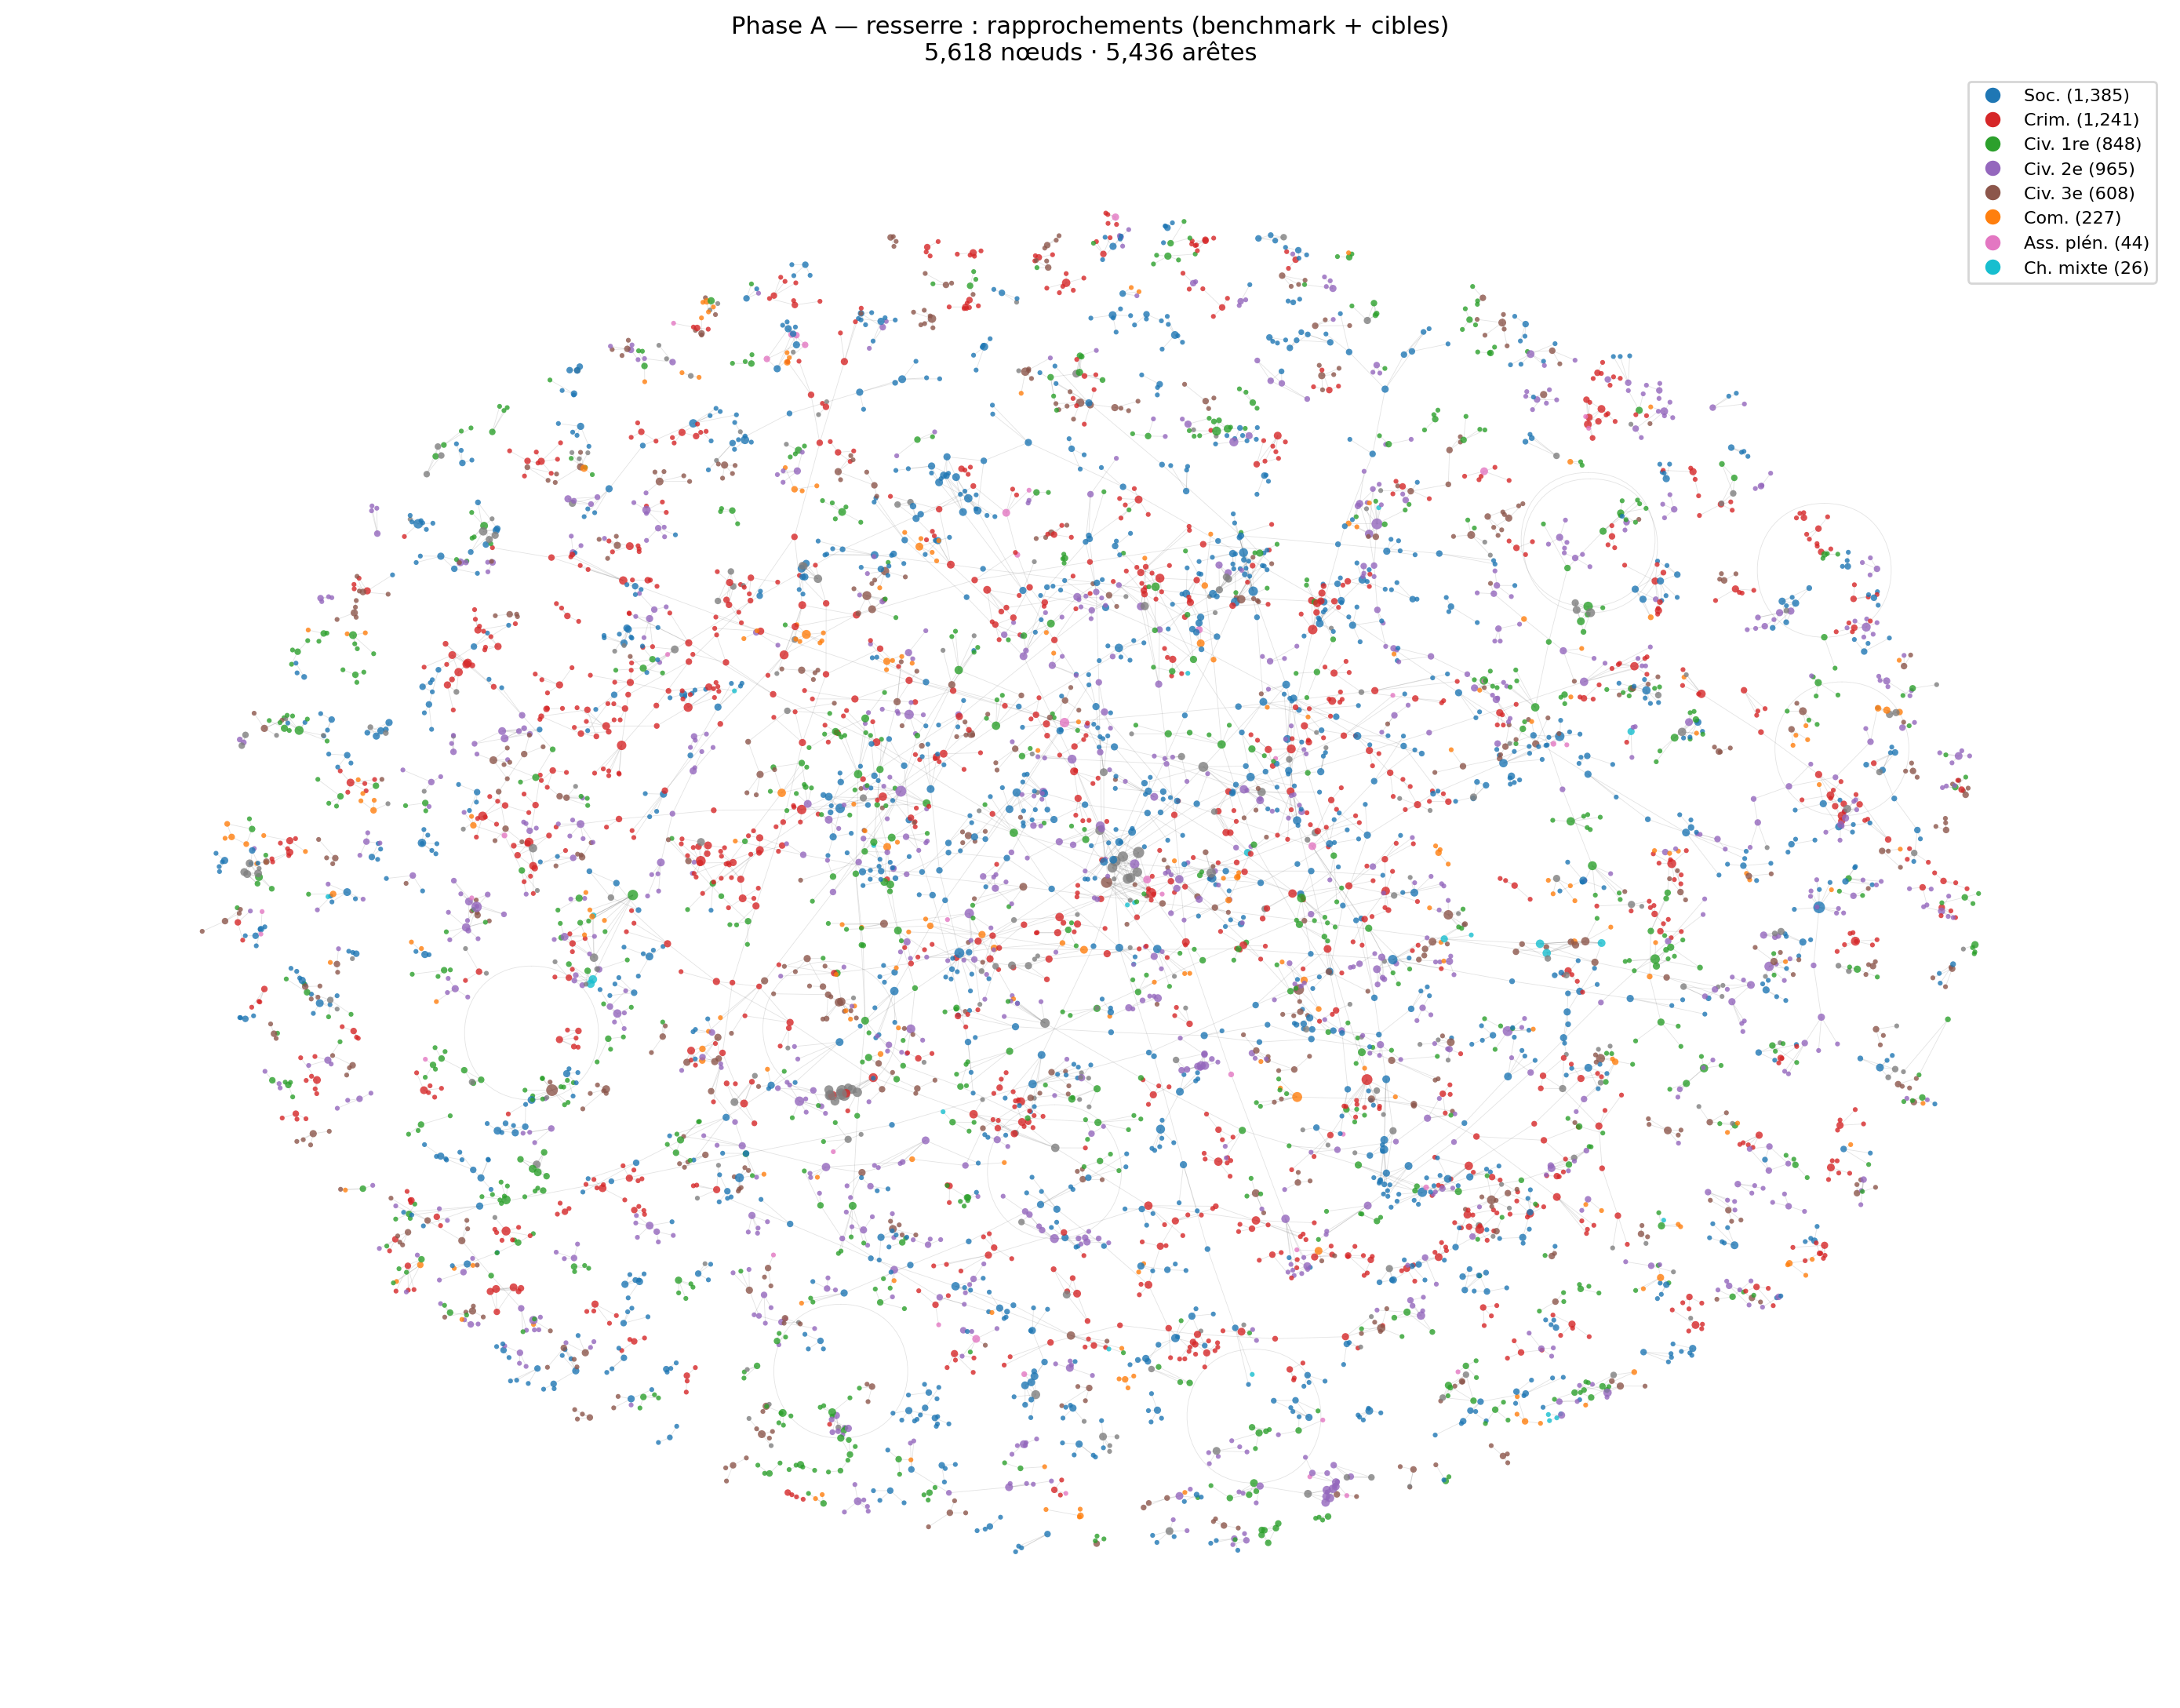
\includegraphics[width=\linewidth]{../../05-Technique/benchmark/data/figures/A1-rapp-resserre.png}

    \vspace{0.2em}
    \scriptsize\textit{Galaxie fragmentée --- 884 composantes éparpillées, pas de centre.}

    \column{0.48\textwidth}
    \centering
    \textbf{B1 --- Bipartite JP $\times$ Articles}

    \vspace{0.3em}
    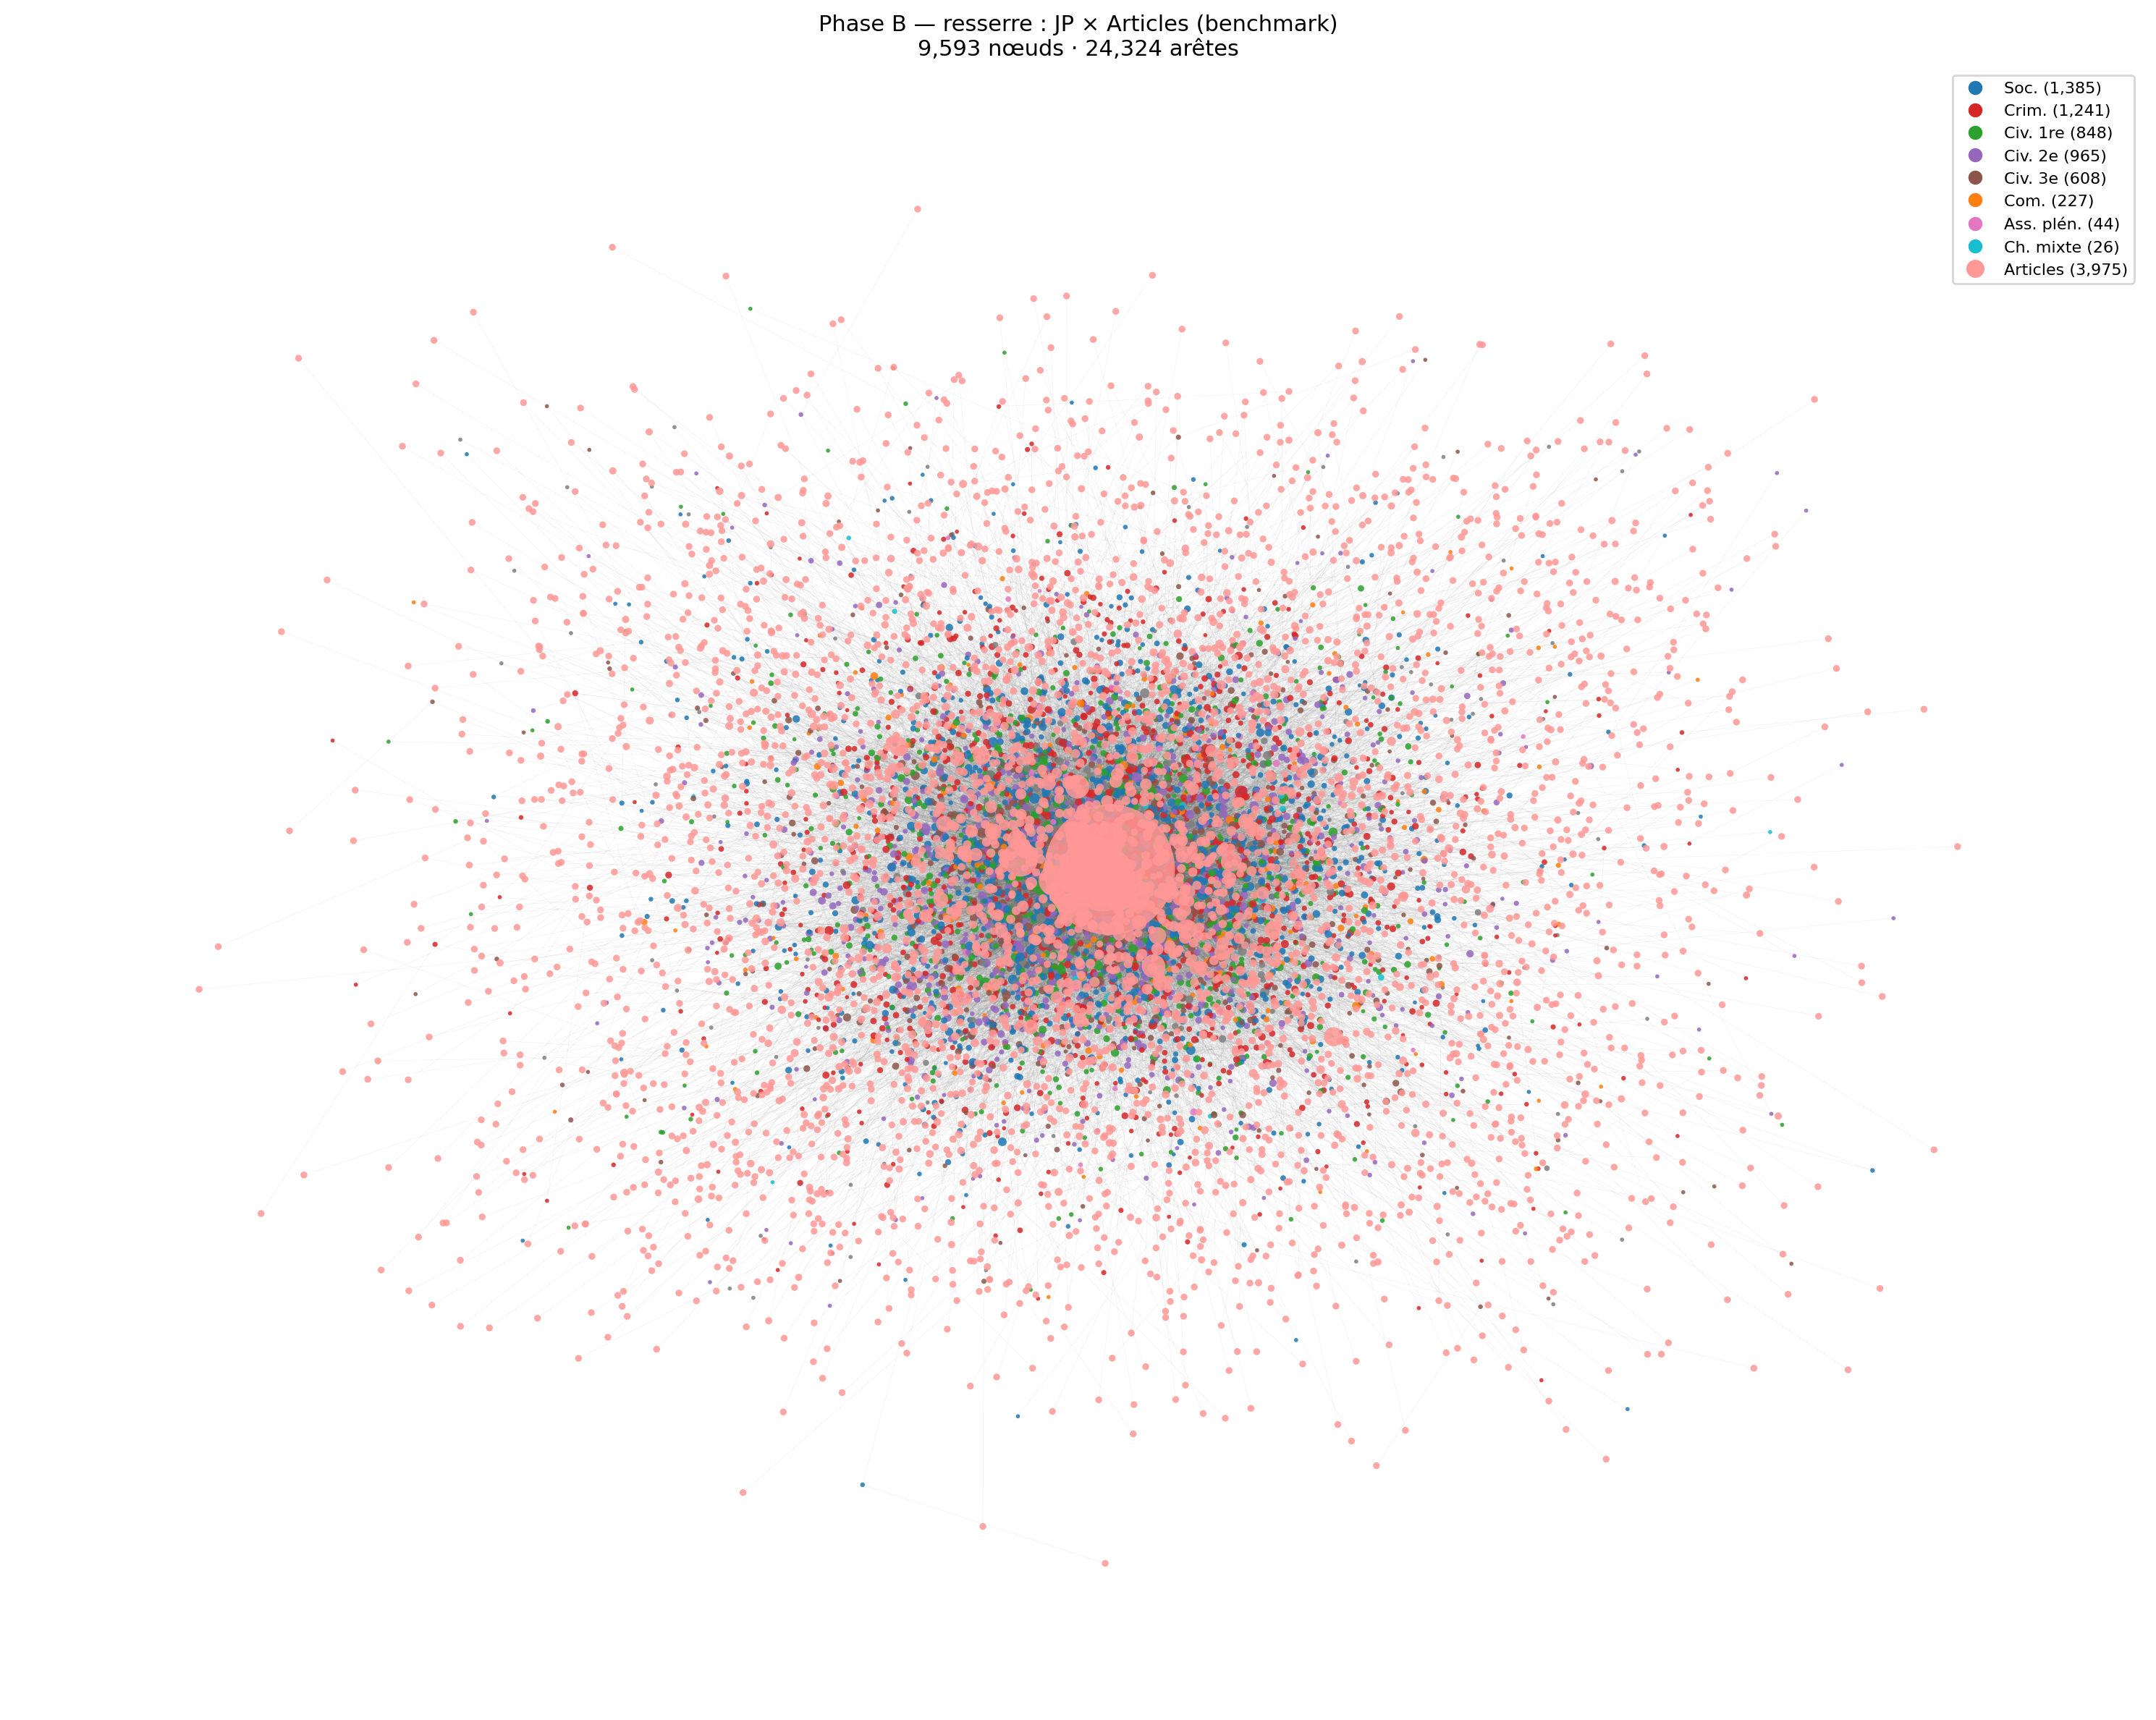
\includegraphics[width=\linewidth]{../../05-Technique/benchmark/data/figures/B1-bip-resserre.png}

    \vspace{0.2em}
    \scriptsize\textit{Noyau rouge dense = articles hubs. Structure centre-périphérie.}
  \end{columns}

  \vspace{0.5em}
  \keybox{\small Même périmètre (1\,532 arrêts-sources), deux topologies radicalement différentes. \textbf{Démonstration empirique directe que le KG doit inclure les articles pour donner de la connectivité.}}
\end{frame}

% ============================================================
\section{Découverte méthodologique}

\begin{frame}{Découverte émergente --- la renumérotation 2016}
  Le graphe bipartite expose un \textbf{problème d'identité temporelle des articles}.

  \vspace{0.3em}
  \footnotesize
  \begin{tabular}{@{}l l l@{}}
    \toprule
    \textbf{Avant 2016} & \textbf{Depuis 2016} & \textbf{Règle} \\
    \midrule
    \texttt{code\_civil:1382} & \texttt{code\_civil:1240} & Responsabilité délictuelle \\
    \texttt{code\_civil:1134} & \texttt{code\_civil:1103 / 1104 / 1193} & Force obligatoire du contrat \\
    \texttt{code\_civil:1147} & \texttt{code\_civil:1231-1} & Responsabilité contractuelle \\
    \bottomrule
  \end{tabular}

  \vspace{0.5em}
  \textbf{Conséquence structurelle}
  \begin{itemize}\footnotesize
    \item Deux arrêts sur la \textbf{même règle juridique} publiés avant/après 2016 ne sont \textbf{pas connectés} dans le graphe via cet article
    \item Faux clivage --- centralité sous-estimée pour les articles historiques
  \end{itemize}

  \vspace{0.3em}
  \textbf{Implication directe pour M5 (Temporalité)}
  \keybox{\small Résolution du problème = \textbf{prérequis} pour M5. Solution retenue : ajouter des arêtes \texttt{recodified\_as} --- fidélité historique préservée + navigabilité augmentée.}
\end{frame}

% ============================================================
\section{Bilan et prochaines étapes}

\begin{frame}{Bilan semaine 2}
  \textbf{Livrables consolidés}

  \footnotesize
  \begin{tabular}{@{}l l@{}}
    \toprule
    Benchmark CRFPA (M1')     & 38 questions, 681 points de rubrique \\
    Benchmark Rapprochements (M3) & 1\,532 questions, 5\,832 rapprochements GT \\
    Graphes Phase A           & 3 périmètres (pickle + GraphML) \\
    Graphes Phase B           & 3 périmètres (infra pour config C) \\
    Figures                   & 6 PNG 200 DPI \\
    Scripts                   & 4 pipelines Python monolithiques \\
    Documentation Obsidian    & 2 journaux + 4 design docs \\
    \bottomrule
  \end{tabular}

  \vspace{0.5em}
  \textbf{Chiffres consolidés}
  \begin{itemize}\footnotesize
    \item 553\,k arrêts CC scannés
    \item 18\,900 arêtes \texttt{rapproche} parsables
    \item 1{,}2\,M arêtes \texttt{cite} (Decision $\to$ Article)
    \item 33\,k articles canoniques uniques
    \item \textbf{1\,570 questions de benchmark au total à la fin de la semaine}
  \end{itemize}
\end{frame}

\begin{frame}{État d'avancement module par module}
  \footnotesize
  \renewcommand{\arraystretch}{1.15}
  \begin{tabular}{@{}l l l@{}}
    \toprule
    \textbf{Module} & \textbf{Statut} & \textbf{Source} \\
    \midrule
    M1  --- Principe QA             & \textcolor{ok}{Disponible (Les-Audits-Affaires, 2\,670 cas)} & Alhajar 2025 \\
    M1' --- CRFPA (complément)      & \textcolor{ok}{\textbf{Livré (38 Q, triangulé)}}   & CNB + Cap'Barreau + IEJ \\
    M2  --- Applied QA              & En cours                                           & Cases Hector + manuel \\
    M3  --- Multi-saut              & \textcolor{ok}{\textbf{Livré (1\,532 Q)}}          & Judilibre \texttt{rapprochements} \\
    M4  --- QCM (V4 revirement)     & Semaine 3                                          & Génération auto depuis graphe B \\
    M5  --- Temporalité             & Bloqué sur renumérotation 2016                     & À débloquer \\
    M6  --- Interprétation arrêt    & \textcolor{ok}{5 cas gold MVP}                     & Pattern Hector AI \\
    \bottomrule
  \end{tabular}
\end{frame}

\begin{frame}{Prochaines étapes --- direction jalon 16 mai}
  \textbf{Semaine 3 (22-28 avril)}
  \begin{itemize}\footnotesize
    \item \textbf{Baselines B1} : LLM seul sur CRFPA + Rapprochements \\ (Gemma 3, Mistral, Saul-Instruct, GPT-5, Claude Opus)
    \item \textbf{Baselines B2} : LLM + RAG vectoriel Légifrance (\texttt{multilingual-e5-large})
    \item Script de validation Judilibre sur les 188 JP du benchmark CRFPA
    \item Générateur M4 V4 (QCM revirement) depuis graphe Phase B
  \end{itemize}

  \vspace{0.3em}
  \textbf{Semaines 4-5}
  \begin{itemize}\footnotesize
    \item Analyse Louvain sur le graphe bipartite $\rightarrow$ clusters thématiques automatiques
    \item Résolution de la renumérotation 2016 $\rightarrow$ prérequis pour M5
    \item Élargissement CRFPA aux sessions 2022-2024
  \end{itemize}

  \vspace{0.3em}
  \keybox{\small \textbf{Jalon superviseur 16 mai} : premier scoreboard B1 vs B2 sur les benchmarks CRFPA + Rapprochements.}
\end{frame}

\begin{frame}{Points de décision pour le superviseur}
  \begin{enumerate}
    \item \textbf{Stratégie renumérotation 2016} : confirmer l'ajout d'arêtes \texttt{recodified\_as} avant B1, ou différer en v2 du graphe ?
    \item \textbf{Priorité semaine 3} : lancer B1 + B2 sur les 2 benchmarks \textit{ou} construire M4 V4 (QCM revirement) en premier ?
    \item \textbf{Extension CRFPA} : intégrer les sessions 2022-2024 pour monter à $\sim$100 Q, ou geler à 38 Q et passer à M2/Applied QA ?
    \item \textbf{Timing du gel benchmark} $\leftrightarrow$ premier scoreboard : avril ou mai ?
  \end{enumerate}

  \vspace{0.7em}
  \keybox{\small Ces 4 décisions déterminent le contenu exact du scoreboard du 16 mai.}
\end{frame}

% ============================================================
\appendix

\begin{frame}{Annexe A --- Format canonique du graphe}
  \textbf{N\oe ud Decision (JP)}
  \begin{block}{}
    \scriptsize\texttt{\{type: "decision", pourvoi\_norm: "10-87525", id\_judilibre: "61403186...", \\
    ecli: "ECLI:FR:CCASS:2011:CR01803", chamber: "Crim.", date: "2011-03-22", \\
    solution: "Rejet", publication: "Publié au Bulletin", is\_benchmark\_src: True\}}
  \end{block}

  \textbf{N\oe ud Article} (format \texttt{Format-Fondement-Juridique})
  \begin{block}{}
    \scriptsize\texttt{\{type: "article", pair\_key: "code\_civil:1240", \\
    code\_slug: "code\_civil", article\_num: "1240", n\_citations\_corpus: 1030\}}
  \end{block}

  \textbf{Arêtes}
  \begin{itemize}\footnotesize
    \item \texttt{rel="rapproche"} : Decision $\to$ Decision (Phase A)
    \item \texttt{rel="cite"}      : Decision $\to$ Article (Phase B)
  \end{itemize}
\end{frame}

\begin{frame}{Annexe B --- Pipeline synoptique}
  \centering
  \begin{tikzpicture}[scale=0.85, transform shape,
      src/.style={rectangle, rounded corners, draw=accent, fill=accentsoft, thick, minimum width=3cm, minimum height=0.6cm, font=\scriptsize},
      proc/.style={rectangle, draw=accent!80, thick, minimum width=3.2cm, minimum height=0.6cm, font=\scriptsize, fill=white},
      out/.style={rectangle, rounded corners, draw=ok, fill=green!8, thick, minimum width=3.2cm, minimum height=0.6cm, font=\scriptsize}]

    % Sources
    \node[src] (cnb)  at (0,3)  {CNB sujets (2024, 2025)};
    \node[src] (cap)  at (0,2.2){Cap'Barreau grilles};
    \node[src] (iej)  at (0,1.4){IEJ Strasbourg copies};
    \node[src] (judi) at (0,-0.4){Judilibre enrichie (5 Go)};

    % Traitements
    \node[proc] (tri)   at (5.5,2.2) {Triangulation (10 subagents)};
    \node[proc] (scan)  at (5.5,-0.4){Scan streaming 3 passes};
    \node[proc] (idx)   at (5.5,-1.2){Index pourvoi $\to$ id};
    \node[proc] (pairs) at (5.5,-2.0){+ \texttt{code\_article\_pairs}};

    % Outputs
    \node[out] (crfpa)    at (11,2.2){38 Q CRFPA};
    \node[out] (rapp)     at (11,-0.4){1\,532 Q rapprochements};
    \node[out] (graphA)   at (11,-1.2){Graphes Phase A};
    \node[out] (graphB)   at (11,-2.0){Graphes Phase B};

    \draw[-{Stealth}, thick] (cnb.east) -- (tri.west);
    \draw[-{Stealth}, thick] (cap.east) -- (tri.west);
    \draw[-{Stealth}, thick] (iej.east) -- (tri.west);
    \draw[-{Stealth}, thick] (tri) -- (crfpa);

    \draw[-{Stealth}, thick] (judi.east) -- (scan.west);
    \draw[-{Stealth}, thick] (scan) -- (rapp);
    \draw[-{Stealth}, thick] (scan) -- (idx);
    \draw[-{Stealth}, thick] (idx)  -- (graphA);
    \draw[-{Stealth}, thick] (idx)  -- (pairs);
    \draw[-{Stealth}, thick] (pairs)-- (graphB);
  \end{tikzpicture}

  \vspace{0.5em}
  \footnotesize\textit{Résultat : 1\,570 questions de benchmark + 6 graphes + 6 figures.}
\end{frame}

\begin{frame}{Annexe C --- Carte des papiers mobilisés}
  \footnotesize
  \begin{tabular}{@{}p{2.8cm} p{4.5cm} p{6.5cm}@{}}
    \toprule
    \textbf{Rôle} & \textbf{Papier} & \textbf{Contribution} \\
    \midrule
    Format rubrique        & OpenAI HealthBench (2025)       & Strates de poids différentiés \\
    Format rubrique        & Shi \textit{et al.} PLawBench (2026) & Rubric-based evaluation \\
    M1 socle               & Alhajar (LegMLAI) 2025         & 2\,670 cas FR --- socle M1 \\
    M6 socle               & Hector AI (interne)             & Pattern Judge-on-Judge + 7 dimensions \\
    Taxonomie d'erreurs    & Butler-Butler Isaacus 2026      & Métriques $g_i / r_i / c_i$ \\
    Contexte RAG FR        & Harvard LIL 2024                & Diagnostic du RAG vectoriel FR \\
    Référence KG juridique & Belikov-Raoult 2025             & Premier KG de la jurisprudence FR \\
    Référence GraphRAG     & Microsoft 2024                  & Architecture de référence \\
    Référence KG + LLM     & Guha 2026                       & Argumentaire KG $>$ RAG pur \\
    \bottomrule
  \end{tabular}
\end{frame}

\begin{frame}
  \begin{center}
    \vspace{1em}
    {\Huge \textbf{Merci}}

    \vspace{1em}
    {\Large Questions ?}

    \vspace{2em}
    \footnotesize\textit{Toutes les données, scripts et design docs sont versionnés dans le vault Obsidian + Git.}
  \end{center}
\end{frame}

\end{document}
